\section{Process and Results}

\subsection{Capital Asset Pricing Model}
To determine the CAPM for each asset, we must first calculate the Risk-Free Rate (\(R_f\)), Expected Market Return (\(R_m\)), Beta (\(\beta\)) for each asset. Below lays out the steps

1. Risk-Free Rate (\(R_f\))

The risk-free rate is typically the return on government bonds, such as U.S. Treasury bills. We decided to use the average risk-free rate over our analysis period for CBOE Interest Rate 10 Year T No \cite{YahooFinanceTNX}

2. Expected Market Return (\(R_m\))

To measure the expected market return, we decided to align our focus to the cryptocurrency market. The expected market return is the average return of a broad cryptocurrency market index, and we used the Bitwise 10 Crypto Index Fund (BITW) \cite{bitw}.

3. Beta Calculation (\(\beta\))

Beta measures the volatility of an asset relative to the market. 

\begin{itemize}
    \item Obtained historical daily prices for each asset and the chosen market index.
    \item Computed the daily returns for each asset and the market index.
    \item Performed a linear regression with the asset returns as the dependent variable and the market index returns as the independent variable. The slope of the regression line is the beta.
\end{itemize}

4. Market Risk Premium (\(R_m - R_f\))

The market risk premium is the difference between the expected market return and the risk-free rate.

Combining each component into the CAPM Model, we obtained the following results.

\begin{table}[h]
\centering
\begin{tabular}{|c|c|c|c|}
\hline
\textbf{Asset} & \textbf{Beta} & \textbf{Market Risk Premium} & \textbf{Expected Return (CAPM)} \\
\hline
AAPL & 0.1489 & -0.0346 & 0.0294 \\
MSFT & 0.1469 & -0.0346 & 0.0295 \\
AMZN & 0.2194 & -0.0346 & 0.0270 \\
GOOGL & 0.1653 & -0.0346 & 0.0289 \\
TSLA & 0.2734 & -0.0346 & 0.0251 \\
SPY & 0.1084 & -0.0346 & 0.0308 \\
DJI & 0.0089 & -0.0346 & 0.0343 \\
AGG & 0.0115 & -0.0346 & 0.0342 \\
VNQ & 0.0884 & -0.0346 & 0.0315 \\
GLD & 0.0195 & -0.0346 & 0.0339 \\
USO & 0.0408 & -0.0346 & 0.0332 \\
SLV & 0.0671 & -0.0346 & 0.0323 \\
PSP & 0.1596 & -0.0346 & 0.0291 \\
BTC-USD & 0.4680 & -0.0346 & 0.0184 \\
ETH-USD & 0.5448 & -0.0346 & 0.0157 \\
SOL-USD & 0.7253 & -0.0346 & 0.0095 \\
BNB-USD & 0.3944 & -0.0346 & 0.0209 \\
XRP-USD & 0.5699 & -0.0346 & 0.0149 \\
TON-USD & 0.4154 & -0.0346 & 0.0202 \\
DOGE-USD & 0.4995 & -0.0346 & 0.0173 \\
ADA-USD & 0.5541 & -0.0346 & 0.0154 \\
SHIB-USD & 0.5231 & -0.0346 & 0.0165 \\
AVAX-USD & 0.6062 & -0.0346 & 0.0136 \\
\hline
\end{tabular}
\caption{CAPM Estimates for Various Assets}
\label{tab:capm}
\end{table}


More information can be found in appendix, please refer to \ref{appendix:capm_details}.

\begin{figure}
    \centering
    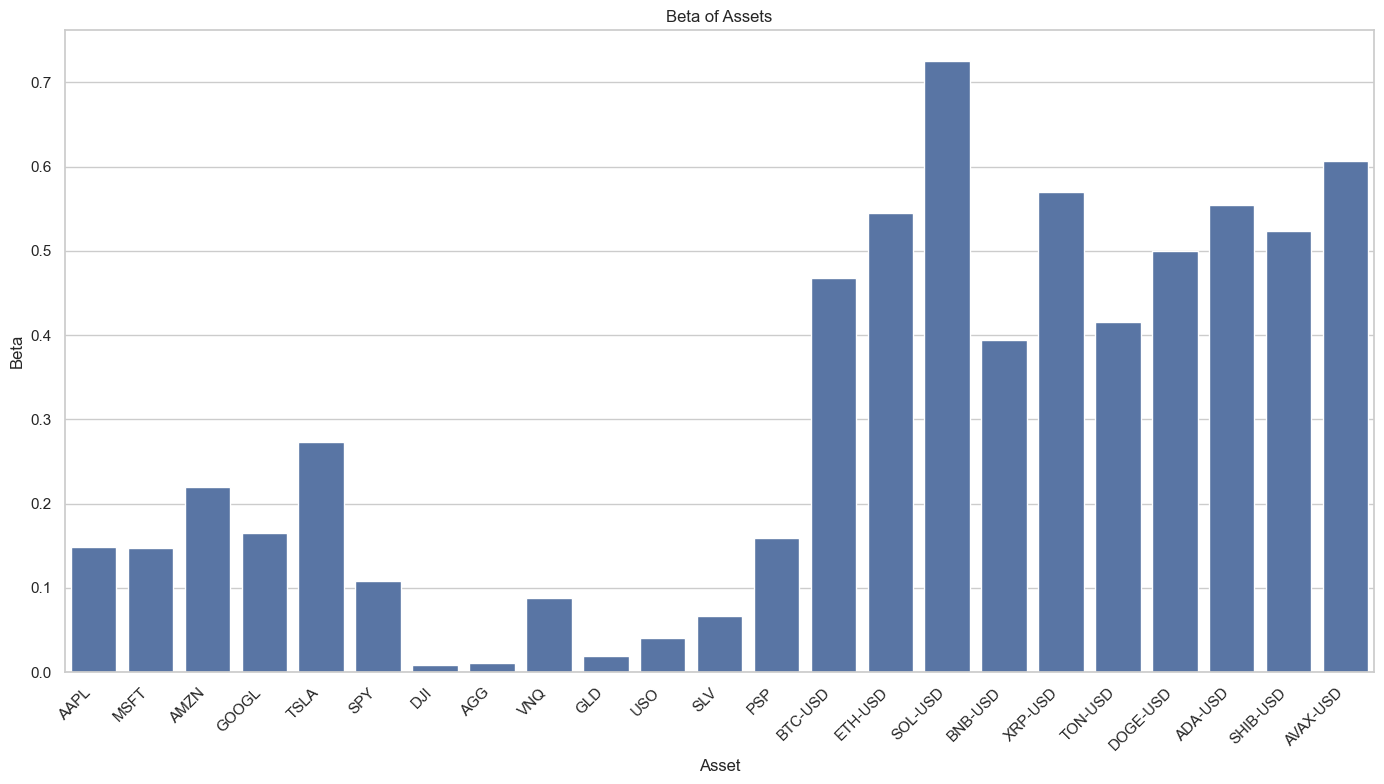
\includegraphics[width=\textwidth]{./code/risk-and-return-analysis/capm/beta_assets.png}
    \caption{Beta of Assets Relative to BITW}
    \label{fig:beta}
\end{figure}

\begin{figure}
    \centering
    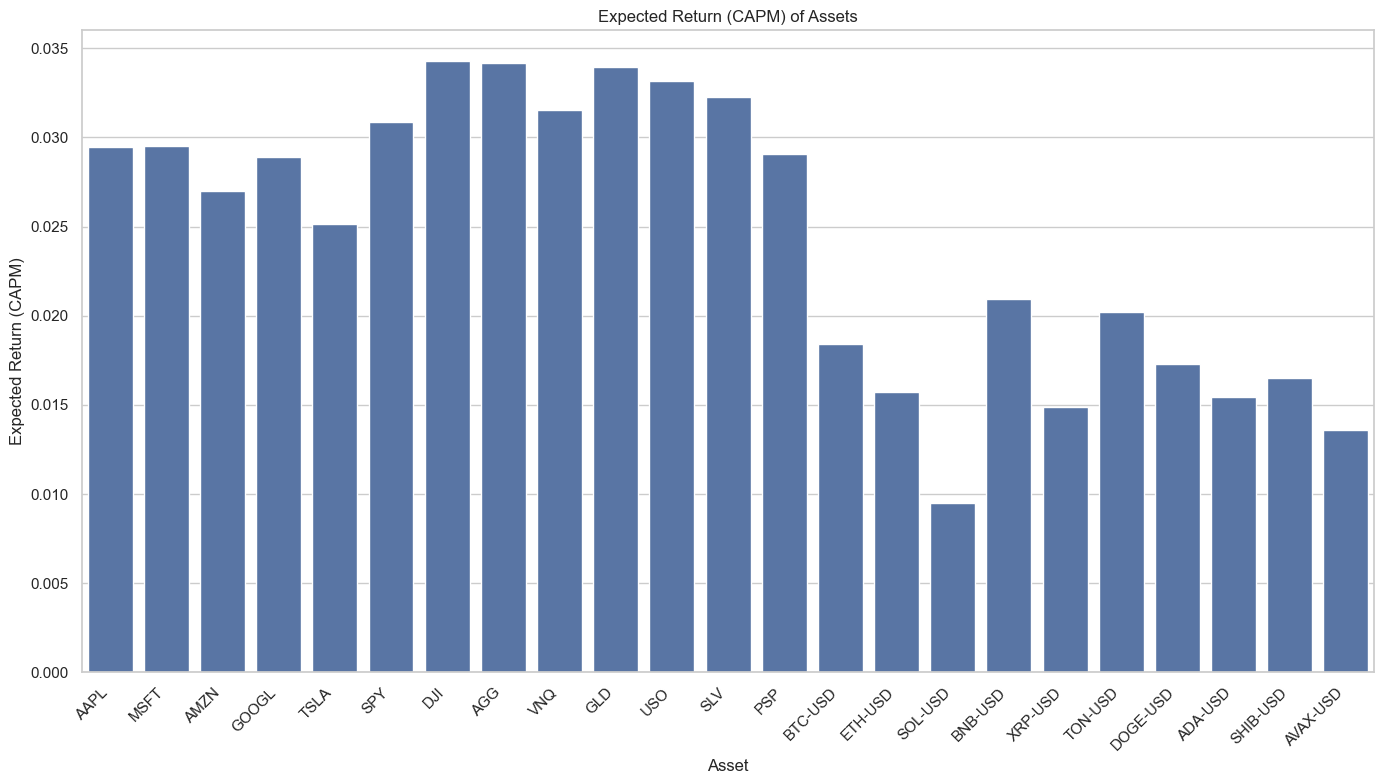
\includegraphics[width=\textwidth]{./code/risk-and-return-analysis/capm/exp_return_assets.png}
    \caption{Expected Return of Assets Relative to BITW}
    \label{fig:exp_return}
\end{figure}


\subsection{GARCH Model}

To investigate the time-varying volatility of different financial assets via the GAR Model, we first calculated the daily returns of each asset. Next, we specified and fitted a GARCH(1,1) model to the return data for each asset. This model choice is common in finance for capturing volatility clustering. After fitting the models, we evaluated their performance using various criteria. This included examining summary statistics, such as the Akaike Information Criterion (AIC) and Bayesian Information Criterion (BIC), to assess model fit and complexity. Additionally, we analyzed residuals to ensure they exhibited characteristics of white noise and conducted stationarity tests to validate model assumptions. Finally, we performed out-of-sample forecasting to assess the model's predictive ability.

\begin{figure}
    \centering
    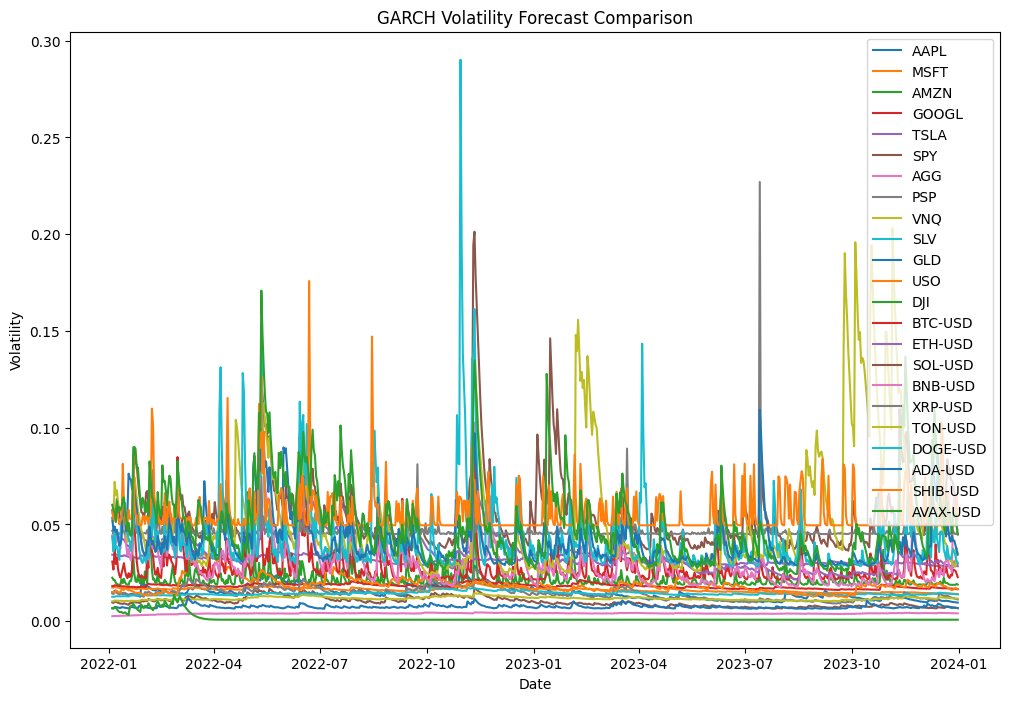
\includegraphics[width=\textwidth]{code/volatility-analysis/garch-with-mulit-assets/garch_forecast.png}
    \caption{GARCH Volatility Forecast}
    \label{fig:exp_return}
\end{figure}

\begin{figure}
    \centering
    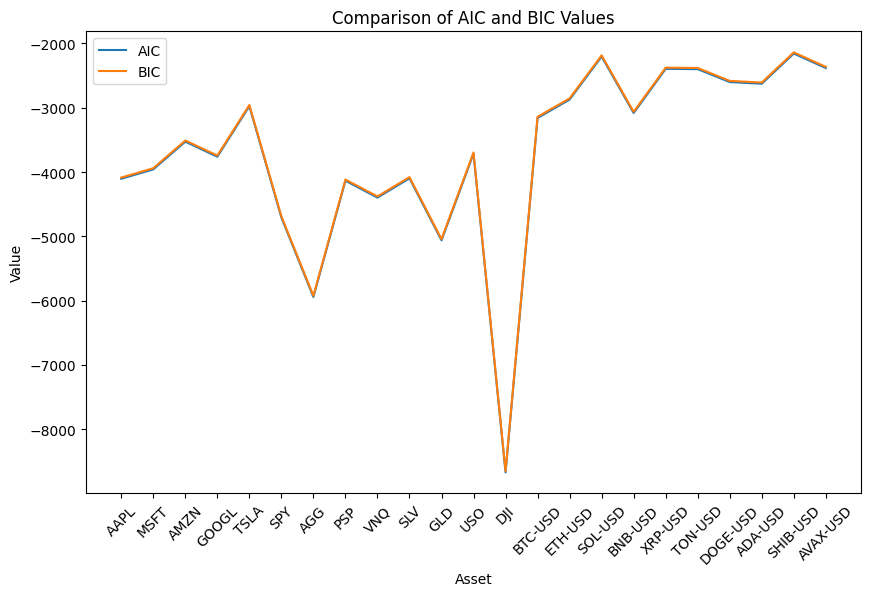
\includegraphics[width=\textwidth]{code/volatility-analysis/garch-with-mulit-assets/aic_bic.png}
    \caption{Comparison between AIC and BIC Values}
    \label{fig:exp_return}
\end{figure}

\begin{figure}
    \centering
    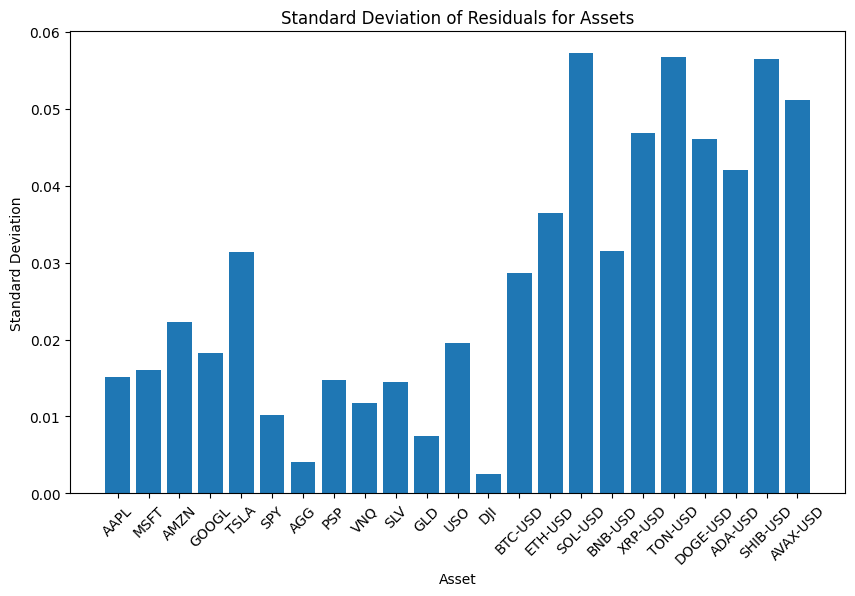
\includegraphics[width=\textwidth]{code/volatility-analysis/garch-with-mulit-assets/standard_deviation.png}
    \caption{Standard Deviation of Residuals}
    \label{fig:exp_return}
\end{figure}



\subsection{Valuation}

% For cryptocurrencies:
% \[
% \text{Intrinsic Value} = \frac{P \times Q}{V}
% \]

% \begin{figure}
%     \centering
%     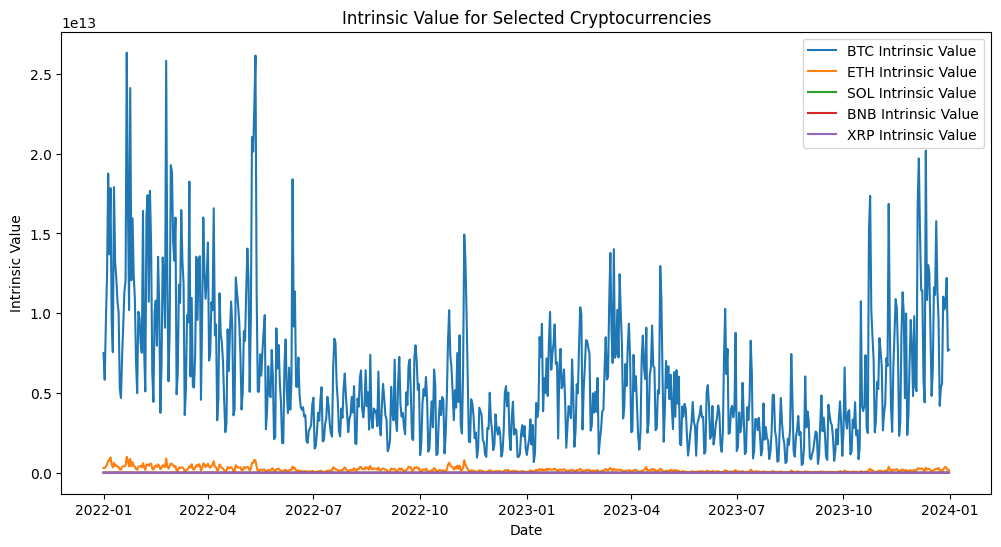
\includegraphics[width=0.8\textwidth]{./code/valuation-techniques/intrinsic_value.png}
%     \caption{Intrinsic Value}
%     \label{fig:beta}
% \end{figure}

\begin{figure}
    \centering
    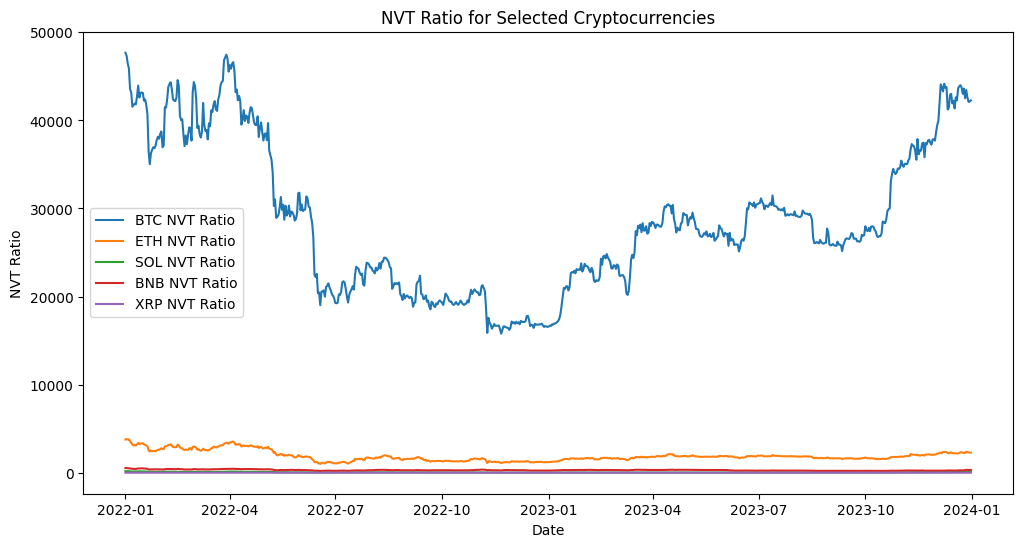
\includegraphics[width=0.8\textwidth]{code/valuation-techniques/nvt_ratio.png}
    \caption{Network Value to Transactions Ratios}
    \label{fig:beta}
\end{figure}

We have to make some assumptions or gather data for $V$ (velocity), $P$ (price level), and $Q$ (transaction volume).

\subsection{LSTM Model}

Preprocessing Steps

Historical price data for the top 10 cryptocurrencies were fetched using the yfinance library, covering the period from January 1, 2022, to January 1, 2024.

The MinMaxScaler from scikit-learn\cite{scikit-learn} was used to normalize the 'Adj Close' price data to a range between 0 and 1. This is crucial for LSTM models, which are sensitive to the scale of input data.

\subsubsection{Model Architecture and Key Values}

In our research, we developed a Bidirectional Long Short-Term Memory (LSTM) model for time series forecasting. Below is a detailed breakdown of the key values and components of our model:

\begin{itemize}
    \item {Sequence Length (SEQ\_LEN)}: 100
    \item {Dropout Rate (DROPOUT)}: 0.2
    \item {Window Size (WINDOW\_SIZE)}: \(SEQ_LEN - 1 = 99\)
    \item {Batch Size (BATCH\_SIZE)}: 64
\end{itemize}

\subsubsection{Model Layers and Structure}

\begin{enumerate}
    \item {Input Layer}:
    \begin{itemize}
        \item Shape: (WINDOW\_SIZE, Number of Features in Input)
        \item Key Value: \texttt{input\_shape = (WINDOW\_SIZE, X\_train.shape[-1])}
    \end{itemize}

    \item {First Bidirectional LSTM Layer}:
    \begin{itemize}
        \item Units: WINDOW\_SIZE = 99
        \item Return Sequences: True
        \item Key Value: \texttt{model.add(Bidirectional(LSTM(WINDOW\_SIZE, return\_sequences=True)))}
    \end{itemize}

    \item {First Dropout Layer}:
    \begin{itemize}
        \item Rate: DROPOUT = 0.2
        \item Key Value: \texttt{model.add(Dropout(rate=DROPOUT))}
    \end{itemize}

    \item {Second Bidirectional LSTM Layer}:
    \begin{itemize}
        \item Units: WINDOW\_SIZE * 2 = 198
        \item Return Sequences: True
        \item Key Value: \texttt{model.add(Bidirectional(LSTM(WINDOW\_SIZE * 2, return\_sequences=True)))}
    \end{itemize}

    \item {Second Dropout Layer}:
    \begin{itemize}
        \item Rate: DROPOUT = 0.2
        \item Key Value: \texttt{model.add(Dropout(rate=DROPOUT))}
    \end{itemize}

    \item {Third Bidirectional LSTM Layer}:
    \begin{itemize}
        \item Units: WINDOW\_SIZE = 99
        \item Return Sequences: False
        \item Key Value: \texttt{model.add(Bidirectional(LSTM(WINDOW\_SIZE, return\_sequences=False)))}
    \end{itemize}

    \item {Dense Layer}:
    \begin{itemize}
        \item Units: 1
        \item Key Value: \texttt{model.add(Dense(units=1))}
    \end{itemize}

    \item {Activation Layer}:
    \begin{itemize}
        \item Activation Function: Linear
        \item Key Value: \texttt{model.add(Activation('linear'))}
    \end{itemize}
\end{enumerate}

\section*{Model Compilation}

\begin{itemize}
    \item Loss Function: Mean Squared Error
    \item Optimizer: Adam
    \item Key Value: \texttt{model.compile(loss='mean\_squared\_error', optimizer='adam')}
\end{itemize}

\section*{Model Training Parameters}

\begin{itemize}
    \item Epochs: 50
    \item Batch Size: BATCH\_SIZE = 64
    \item Shuffle: False
    \item Validation Split: 10\%
    \item Key Value: \texttt{model.fit(X\_train, y\_train, epochs=50, batch\_size=BATCH\_SIZE, shuffle=False, validation\_split=0.1)}
\end{itemize}

\section*{Summary}

We utilized a Bidirectional LSTM model with three layers of bidirectional LSTMs, each followed by dropout layers to prevent overfitting. The final dense layer with a linear activation function is used for regression. Our model is compiled using the mean squared error loss function and the Adam optimizer, and trained over 50 epochs with a batch size of 64, using 10\% of the training data for validation.

This architecture effectively captures temporal dependencies in both directions, making it suitable for time series forecasting tasks.
